%% Преамбула TeX-файла

% 1. Стиль и язык
\documentclass[utf8x]{G7-32} % Стиль (по умолчанию будет 14pt)
\usepackage[T2A]{fontenc}
\usepackage[russian]{babel}
% Остальные стандартные настройки убраны в preamble.inc.tex.
\sloppy

% Настройки стиля ГОСТ 7-32
% Для начала определяем, хотим мы или нет, чтобы рисунки и таблицы нумеровались в пределах раздела, или нам нужна сквозная нумерация.
\EqInChapter % формулы будут нумероваться в пределах раздела
\TableInChapter % таблицы будут нумероваться в пределах раздела
\PicInChapter % рисунки будут нумероваться в пределах раздела

% Добавляем гипертекстовое оглавление в PDF
\usepackage[
bookmarks=true, colorlinks=true, unicode=true,
urlcolor=black,linkcolor=black, anchorcolor=black,
citecolor=black, menucolor=black, filecolor=black,
]{hyperref}

% Изменение начертания шрифта --- после чего выглядит таймсоподобно.
% apt-get install scalable-cyrfonts-tex

\IfFileExists{cyrtimes.sty}
    {
        \usepackage{cyrtimespatched}
    }
    {
        % А если Times нету, то будет CM...
    }

\usepackage{graphicx}   % Пакет для включения рисунков

% С такими оно полями оно работает по-умолчанию:
% \RequirePackage[left=20mm,right=10mm,top=20mm,bottom=20mm,headsep=0pt]{geometry}
% Если вас тошнит от поля в 10мм --- увеличивайте до 20-ти, ну и про переплёт не забывайте:
\geometry{right=20mm}
\geometry{left=30mm}


% Пакет Tikz
\usepackage{tikz}
\usetikzlibrary{arrows,positioning,shadows}

% Произвольная нумерация списков.
\usepackage{enumerate}

% ячейки в несколько строчек
\usepackage{multirow}

% itemize внутри tabular
\usepackage{paralist,array}


% Настройки листингов.
% 8 Листинги

\usepackage{listings}

% Значения по умолчанию
\lstset{
  basicstyle= \footnotesize,
  breakatwhitespace=true,% разрыв строк только на whitespacce
  breaklines=true,       % переносить длинные строки
%   captionpos=b,          % подписи снизу -- вроде не надо
  inputencoding=koi8-r,
  numbers=left,          % нумерация слева
  numberstyle=\footnotesize,
  showspaces=false,      % показывать пробелы подчеркиваниями -- идиотизм 70-х годов
  showstringspaces=false,
  showtabs=false,        % и табы тоже
  stepnumber=1,
  tabsize=4,              % кому нужны табы по 8 символов?
  frame=single
}

% Стиль для псевдокода: строчки обычно короткие, поэтому размер шрифта побольше
\lstdefinestyle{pseudocode}{
  basicstyle=\small,
  keywordstyle=\color{black}\bfseries\underbar,
  language=Pseudocode,
  numberstyle=\footnotesize,
  commentstyle=\footnotesize\it
}

% Стиль для обычного кода: маленький шрифт
\lstdefinestyle{realcode}{
  basicstyle=\scriptsize,
  numberstyle=\footnotesize
}

% Стиль для коротких кусков обычного кода: средний шрифт
\lstdefinestyle{simplecode}{
  basicstyle=\footnotesize,
  numberstyle=\footnotesize
}

% Стиль для BNF
\lstdefinestyle{grammar}{
  basicstyle=\footnotesize,
  numberstyle=\footnotesize,
  stringstyle=\bfseries\ttfamily,
  language=BNF
}

% Определим свой язык для написания псевдокодов на основе Python
\lstdefinelanguage[]{Pseudocode}[]{Python}{
  morekeywords={each,empty,wait,do},% ключевые слова добавлять сюда
  morecomment=[s]{\{}{\}},% комменты {а-ля Pascal} смотрятся нагляднее
  literate=% а сюда добавлять операторы, которые хотите отображать как мат. символы
    {->}{\ensuremath{$\rightarrow$}~}2%
    {<-}{\ensuremath{$\leftarrow$}~}2%
    {:=}{\ensuremath{$\leftarrow$}~}2%
    {<--}{\ensuremath{$\Longleftarrow$}~}2%
}[keywords,comments]

% Свой язык для задания грамматик в BNF
\lstdefinelanguage[]{BNF}[]{}{
  morekeywords={},
  morecomment=[s]{@}{@},
  morestring=[b]",%
  literate=%
    {->}{\ensuremath{$\rightarrow$}~}2%
    {*}{\ensuremath{$^*$}~}2%
    {+}{\ensuremath{$^+$}~}2%
    {|}{\ensuremath{$|$}~}2%
}[keywords,comments,strings]

% Подписи к листингам на русском языке.
\renewcommand\lstlistingname{\cyr\CYRL\cyri\cyrs\cyrt\cyri\cyrn\cyrg}
\renewcommand\lstlistlistingname{\cyr\CYRL\cyri\cyrs\cyrt\cyri\cyrn\cyrg\cyri}


% Полезные макросы листингов.
% Любимые команды
\newcommand{\Code}[1]{\textbf{#1}}


%For titul
%--------------------------------------
\usepackage{graphicx}
\graphicspath{ {./images/} }
\usepackage{tabularx} % in the preamble
\usepackage[normalem]{ulem}
%--------------------------------------

\begin{document}

\begin{titlepage}
    \thispagestyle{empty}

    \noindent\begin{minipage}{0.05\textwidth}
        
\includegraphics[scale=0.3]{bmstu}
    \end{minipage}
    \hfill
    \begin{minipage}{0.85\textwidth}\raggedleft
        \begin{center}
            \fontsize{10pt}{0.3\baselineskip}\selectfont \textbf{Министерство науки и высшего образования Российской Федерации \\ Федеральное государственное бюджетное образовательное учреждение \\ высшего образования \\ <<Московский государственный технический университет \\ имени Н.Э. Баумана \\ (национальный исследовательский университет)>> \\ (МГТУ им. Н.Э. Баумана)}
        \end{center}
    \end{minipage}

    \begin{center}
        \fontsize{12pt}{0.1\baselineskip}\selectfont
        \noindent\makebox[\linewidth]{\rule{\textwidth}{4pt}} \makebox[\linewidth]{\rule{\textwidth}{1pt}}
    \end{center}

    \begin{flushleft}
        \fontsize{12pt}{0.8\baselineskip}\selectfont

        ФАКУЛЬТЕТ \uline{
            \hfill
            Информатика и системы управления
            \hfill}

        КАФЕДРА \uline{\mbox{\hspace{4mm}}
            \hfill
            Программное обеспечение ЭВМ и информационные технологии
            \hfill}
    \end{flushleft}

    \vfill
    
    \begin{center}
        \fontsize{19pt}{\baselineskip}\selectfont

        \textbf{Отчет по лабораторной работе №1} \\
        \textbf{по теме "Дисассемблирование INT 8h"}
    \end{center}

    \vfill
    
    \begin{tabularx}{\textwidth}{Xcc}
        Студент \uline{Недолужко Д.В.} \\
        Группа \uline{ИУ7-53Б} \\
        Преподаватель \uline{Рязанова Н.Ю.} \\
    \end{tabularx}
    
    \vfill
    
    \begin{center}
        \normalsize Москва \\
        \the\year ~г.
    \end{center}
\end{titlepage}

\frontmatter % выключает нумерацию ВСЕГО; здесь начинаются ненумерованные главы: реферат, введение, глоссарий, сокращения и прочее.

% Команды \breakingbeforechapters и \nonbreakingbeforechapters
% управляют разрывом страницы перед главами.
% По-умолчанию страница разрывается.

% \nobreakingbeforechapters
% \breakingbeforechapters


\mainmatter % это включает нумерацию глав и секций в документе ниже

\chapter{Ассемблерный код}

  \lstinputlisting[
    language={[x86masm]Assembler},
    caption=Обработчик INT 8h,
    basicstyle=\scriptsize
  ]{./listings/int8h.asm}
  
  \lstinputlisting[
    language={[x86masm]Assembler},
    caption=Сопрограмма sub\_1,
    basicstyle=\scriptsize
  ]{./listings/sub_1.asm}

\chapter{Схемы алгоритмов}

  \section{Схема алгоритма обработчика INT 8h}
  
    \begin{center}
      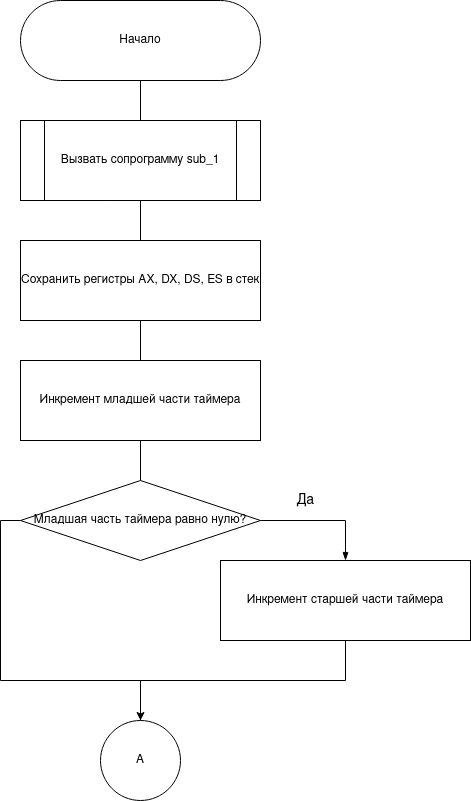
\includegraphics[scale=0.6]{images/scheme-int8h_1.drawio.png}
    \end{center}
    
    \begin{center}
      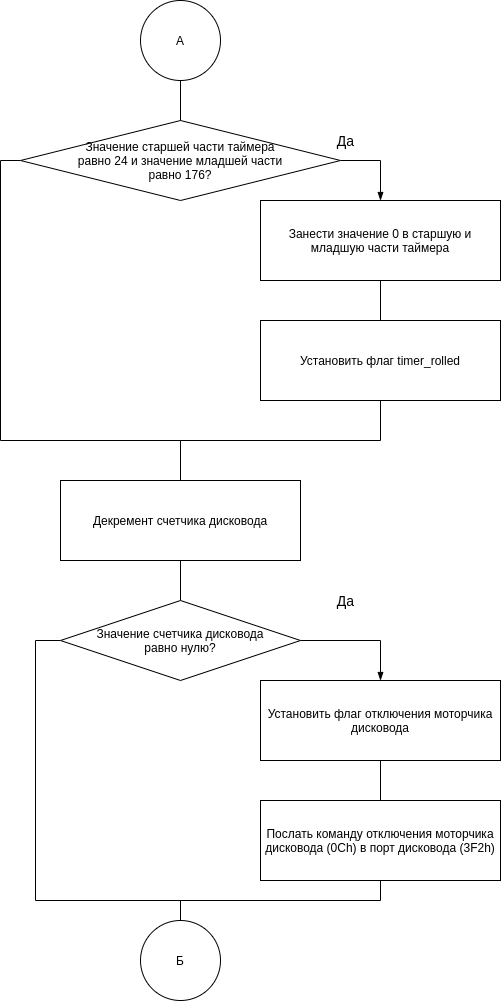
\includegraphics[scale=0.6]{images/scheme-int8h_2.drawio.png}
    \end{center}
    
    \begin{center}
      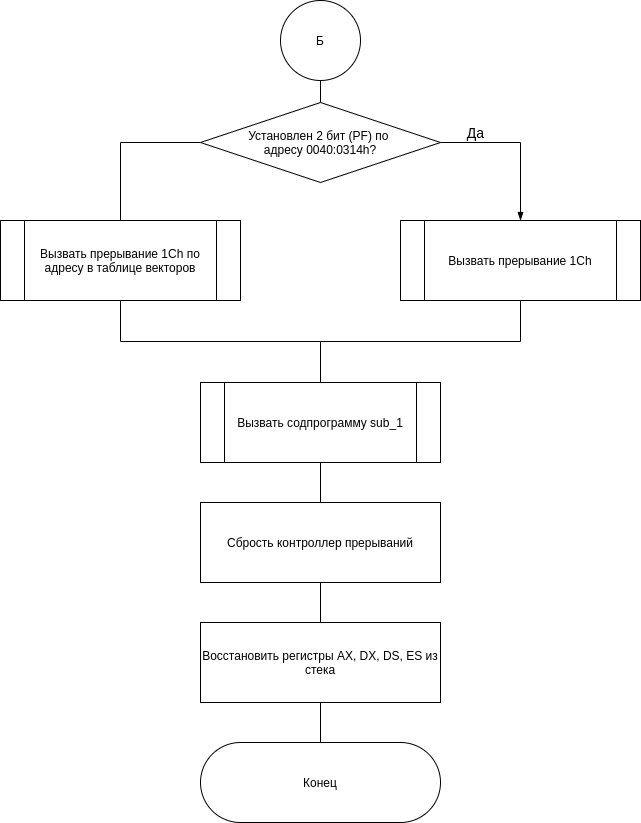
\includegraphics[scale=0.6]{images/scheme-int8h_3.drawio.png}
    \end{center}
  
  \section{Схема алгоритма сопрограммы sub\_01}

    \begin{center}
      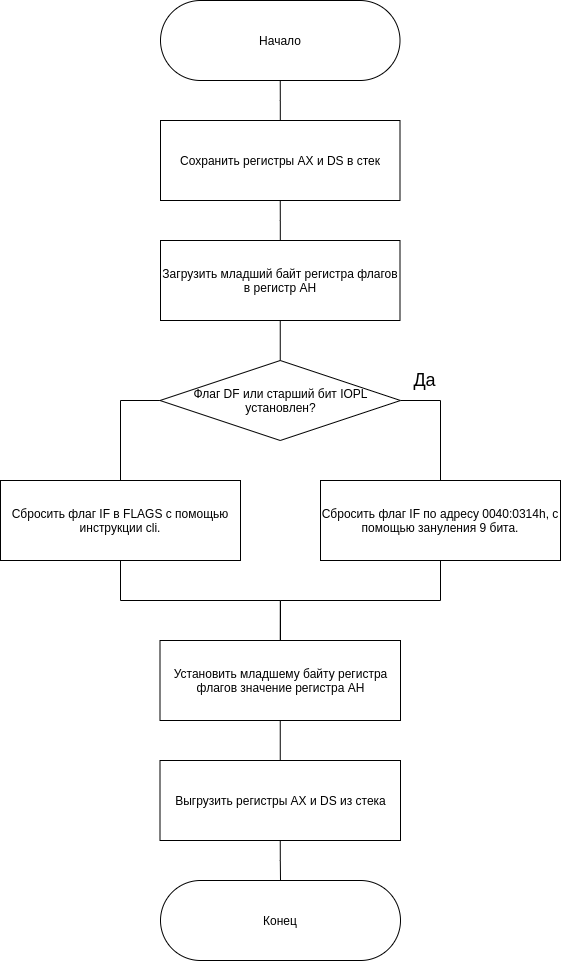
\includegraphics[scale=0.6]{images/scheme-sub_1.drawio.png}
    \end{center}


\end{document}

%%% Local Variables:
%%% mode: latex
%%% TeX-master: t
%%% End:
